\section*{Background}

Understanding complicated networks of biomolecular entities and interactions is essential to solving contemporary problems in modern biology, especially in computational domains such as systems biology \cite{hanahan2011hallmarks}.
Networks of bio-molecular interactions are represented as graph models referred to as \emph{pathways}.
Pathways are curated subsets of a theoretical graph of all known biomolecular entities and events that occur on the cellular level, and a given pathway usually represents a particular biological process, such as mitosis, that is relevant within a given research context.

Pathways are modeled as labeled graphs of entities, relationships, and meta-data. For example, Figure \ref{fig:kvik} shows a typical representation of a pathway as a human curated node-link diagram, where nodes are biological entities and edges represent interactions between them.
An entity is a component of a pathway such as a gene, a gene produce (such as a protein), a complex of proteins, a small biomolecule, or even another pathway.
Edges between vertices in this graph can be directed or undirected, can involve multiple entities in one relationship, and can represent a wide range of biological relationships.
Meta-data can include external information such as experimental data, as well as the \emph{provenance} of the information related to a particular entity or relationship.
Provenance is typically a list of records, such as publications, that reflects the collective history of research related to a given entity or relationship.
Provenance is essential to the field of bioinformatics, as the ``ground truth'' related to any given entity is not immutable, and can be derived from a potentially large and evolving history of research.

\begin{figure}[htb]
  \centering
  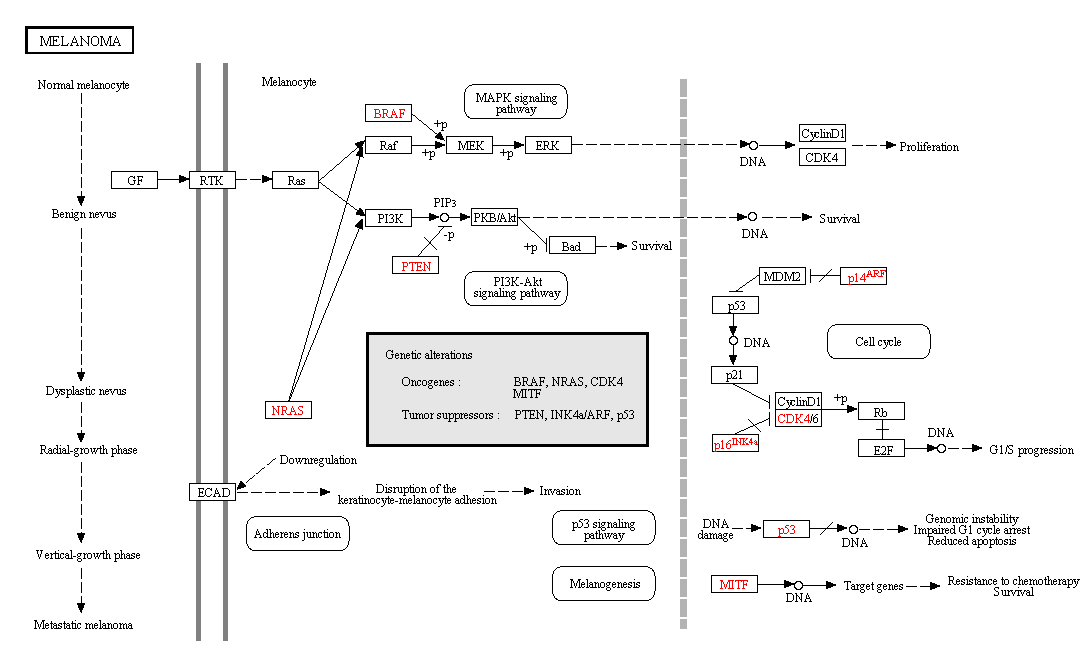
\includegraphics[width=\linewidth]{figures/kegg2}
  \caption{\label{fig:kvik} A view of a typical KEGG diagram. From \cite{Fjukstad2014kvik}.}
\end{figure}

Researchers who work with pathway data are confronted with a number of challenges.
Pathway files may contain hundreds or thousands of entities that are connected by a wide variety of relationship types.
For instance, the \emph{BioPax} specification \hl{citation! http://www.biopax.org/release/biopax-level3-documentation.pdf} contains a ``Transport'' class, which is one of four types of ``Conversion'', which in turn is one of five different types of ``Interaction'', which, finally, is one of four types of ``Entity''.
The \emph{BioPax} schema is itself a reflection of the complexity of information that can exist within bio-chemical pathway datasets.

Participants in a pathway -- genes, proteins, and other molecules within a cell -- can act as inputs or outputs to multiple interactions, and the set of relationships between biochemical interactions inherently includes feedback loops and other complex relationships.
Importantly, reactions and other interactions can have a ``cascading'' effect, where one interaction will inhibit or promote the effect of another.
Molecular activation pathways also have an inherently dynamic quality, which can limit the utility of static (i.e., non-interactive) graph representations \cite{kitano2002systems}.
Understanding these complex and dynamic relationships while also enabling researchers to see higher order patterns is a significant challenge to modern bioinformatics research \cite{saraiya2005visualizing}.

Pathway diagrams are used in two contexts: for the presentation of results, and as an active (and interactive) part of the process of data analysis.
In the presentational sense, pathway diagrams can contextualize a set of biological processes within a cell, and in these contexts will often show the location of cellular membranes and other large cellular structures to help provide a frame of reference for the viewer.
Ideally, a pathway diagram --~when used in a presentational context -- allows a viewer to efficiently understand a complex set of biological relationships.
While pathway diagrams may be useful for presenting and contextualizing a set of results in a research or educational context, they are also an important part of \emph{in situ} analyses.

For example, metabolic activation networks are of critical importance to cancer researchers, who hope to understand -- and potentially disrupt -- malignant cycles of uncontrolled cellular growth, replication, and mediated cell death \cite{cairns2011regulation}.
Effective cancer drug development involves determining how proteins and complexes that are affected by a drug in turn affect important cellular pathways.
In this domain, the ``downstream'' consequences of a particular drug effect are especially important \cite{luo2003targeting}.
Stem-cell researchers can also use pathways as an active part of their research, where the goal is generally to precipitate a desired cellular differentiation into specific cell types \cite{reya2001stem}.
In these contexts, understanding the complex relationships that are encoded in pathway data is paramount.

In the last two decades, as the availability of large stores of data to researchers has increased, analyses that involve hundreds or thousands of genes and gene products have become common.
When analyzing such large and complex data, visual representations can be essential, and in many cases static, non-interactive, representations will fail to adequately convey the dynamic nature of a pathway.
The complexity and amount of information that needs to be incorporated in given diagram can also make static representations cluttered and difficult to interpret.
Thus, modern applications in these domains employ a wide variety of interactive visualization techniques to allow a user to effectively explore and analyze pathway data.

Developing and designing effective visual analytics applications requires a detailed understanding of the visual analysis tasks that will be performed by a user, and the ``user'' in this case is a biological researcher in the midst of some analysis relevant to their domain.
User tasks can thus be designed and understood best through a in-depth understanding of the nature of information needed by the researcher in the course of their analyses.
Some of these tasks may not be known \emph{a priori} and may be exploratory in nature, where an ideal visualization of pathway data could reveal important new insights to a researcher.
A comprehensive understanding of tasks performed by domain researchers in a typical analysis is essential to the design and implementation of an effective visual analytics application.

In this work, we present a description and analysis of tasks and requirements related to the analysis of biological pathway data.
Tasks were derived from interviews with several domain experts in biology.
After an introduction to the structure and content of pathway data, we describe the task taxonomy that was constructed from these interviews.
We also review visual representations of pathway data in the context of our requirements, along with a brief discussion of existing tools which implement those visual representations.
Finally, avenues of future research are considered, along with a brief summary of lessons learned from domain experts.

\subsection*{Biological Pathway Visualization}

Pathway models are an important concept in biological research \cite{cairns2011regulation, luo2003targeting, reya2001stem}.
Visualization techniques and applications are important tools for researchers who work with complex data, and biological pathways are an active area of visualization research.

A number of surveys exist that describe the large number of existing tools for biological network visualization \cite{Suderman2007tools,pavlopoulos2008survey,Gehlenborg2010omics}.
In this paper we highlight some of the more prominent existing tools and techniques that provide support for the tasks described in our taxonomy.
However, this paper is not intended to be a complete survey of biological visualization techniques and applications.
Existing techniques included in this paper include the following: \textit{ChiBe} \cite{Babur2010chibe}, \textit{Entourage} \cite{Lex2013entourage}, \textit{Reactome Pathway Browser} \cite{croft2014reactome}, \textit{VisAnt} \cite{hu2004visant}, \textit{MetaViz} \cite{bourqui2007metabolic}, \textit{VitaPad} \cite{holford2005vitapad}, and \textit{BioFabric} \cite{Longabaugh2012biofabric}.

Node-link diagrams are the nearly-universal choice of visual representation used in existing applications (exceptions to this rule include Biofabric \cite{Longabaugh2012biofabric}).
Cytoscape \cite{cytoscape} is a popular graph visualization application which was originally designed for biological data, and offers many sophisticated plug-ins that have been developed by the research community, including Cerebral\cite{Barsky2008cerebral} and RenoDoI\cite{Vehlow2015}.
However, node-link representations are one of several ways to visualize graph data, and there are alternative visualization techniques which can be applied to pathway data.
For instance, research has shown that matrix visualization techniques outperform node-link diagrams for higher level group based tasks\cite{Ghoniem2004,Henry2007}.
While these matrix techniques are not as effective for certain tasks (such as path-tracing), linked views and hybrid techniques exist, such as NodeTrix \cite{NodeTrix2007}, which combine node-link and matrix representations.

\subsubsection*{Pathway Data Formats}

Pathway data can be stored in a variety of file formats which capture the underlying structure of pathway data.
In particular, \textit{BioPAX} \cite{demir2010biopax}, \textit{KEGG} \cite{kanehisa2000kegg} and \textit{SBML} \cite{Hucka2003} are the most popular file standards for storing the complex graph data structures inherent in pathway data.

All three of these popular formats are XML-based and represent data as an ontology.
\emph{BioPAX}, in particular, was designed to be a general format for biological pathway data across a variety of domain contexts \cite{demir2010biopax}.
Systems Biology Graph Notation (SBGN) \cite{Novere2009} is a visual standard often used to visualize \textit{BioPAX} and \textit{SBML} file formats.
Features particular to SBGN include the definition of multiple edge and node types, as well as allowing edges to connect to more than two nodes, resulting in a hypergraph.
Other formats are used for the visualization of biological pathways that are not specific to the field of biology.
For instance, the \textit{SIF Simple Interaction Format} is used by \textit{Cytoscape} \cite{Shannon2003cytoscape} to represent undirected interactions between participants.

\subsection*{Task Taxonomies}

The field of visual analytics has produced a number of \emph{task taxonomies}, which are written in an effort to understand how the various tasks performed by an analyst and user are related to (and enabled by) different visualization tools and techniques, and, conversely, how visualization tools might inform analytic tasks.
These taxonomies help to clarify the utility of existing techniques while also providing a low-level template for the design and evaluation of new techniques.
Wehrend and Lewis \cite{Wehrend1990} provide one of the earliest visualization task taxonomies, with the goal of ``accelerating progress in scientific visualization'' by allowing researchers to easily find the right visualization technique for a given problem.
Schneiderman \cite{Shneiderman1996} defines a ``task by data type taxonomy'' for information visualization in order to ``to sort out the prototypes and guide researchers to new opportunities.''

These seminal taxonomies were, like many later taxonomies, independent of a specific visualization application domain, and their purpose was to provide a low level description and categorization of the analysis tasks enabled by \textit{any} visualization of data.
These early taxonomies were written as very general classifications of low level analytic tasks related to any data visualization.
In more recent publications, and as visualization research has progressed, task taxonomies have increasingly focused on more constrained subsets of tasks related to particular types of data structures and analytic domains.

More recent taxonomies tend to focus on more narrow categories and domains relevant to visualization.
For instance, Valiati et al. \cite{Valiati2006} provide a taxonomy focused specifically on multidimensional visualizations.
They build on \cite{Wehrend1990}, but focus on tasks uniquely related to multidimensional visualizations (such as parallel coordinates).
Like previous authors, their goal is to guide the choices of visualization and interaction techniques, and also to help support usability testing.
Lee at al \cite{Lee2006} define a taxonomy of graph visualization tasks that are frequently encountered when analyzing graph data.
The stated goal of this work was to improve the evaluation of graph visualization systems by creating a set of common benchmark tasks (which could be used in conjunction with benchmark data sets).
Their taxonomy covers tasks for the analysis of graphs in general, and was inspired by example tasks from several different domains that make regular use of graph data.
The authors build on Amar and Stasko's \cite{Amar2005} list of visual analytic tasks by composing existing low-level tasks into higher-level task compositions, while also proposing additional tasks that are not captured by low-level tasks presented in existing taxonomies.

Several recent taxonomies focus on aspects of graph visualization that extend the work of Lee at al \cite{Lee2006}.
For instance, Ahn et al \cite{Ahn2014} provide a task taxonomy for the analysis of networks that evolve over time, also known as dynamic graphs.
The complex nature of dynamic graph data yields a similarly complex set of analysis tasks, and many of these tasks were not covered by the general graph taxonomy of Lee at al \cite{Lee2006} -- thus, new tasks needed to be specified.
Pretorius et al \cite{Pretorius2014} focus on multivariate graph visualization (where graph elements contain multiple attributes).
Their work builds on the work of both Lee at al \cite{Lee2006} and of Valiati et al. \cite{Valiati2006}, as multivariate networks can be considered a multidimensional dataset.

While these recently-published task taxonomies have focused on particular data structures (or datasets with particular characteristics), to our knowledge the present work is the first taxonomy of tasks written in the context of the domain of biological pathway analysis.

Biological Pathway visualization is a complex application domain that poses many specific analytic challenges that are not encountered in pre-existing task taxonomies.
The data structures underlying biological pathways are dynamic multivariate hyper-graphs, and are more complex than any of those described in previous taxonomies.
The tasks to be completed by biologists are also highly complex, involving many different entity and relationship types, and are not fully covered by the existing taxonomies.

\section*{Methods}

\subsection*{Interviews}

Interviews were conducted with seven domain experts in biology, each of whom works with pathway data in some form.
Those interviewed included one tenured professor, three assistant professors, one researcher at a cancer research institution, one postdoctoral research associate, and one masters student in bioinformatics.
Interviews were loosely structured, but interview questions were designed to elicit a detailed understanding of the tasks performed by the researcher in the course of a typical analysis, as well as an understanding of the type and structure of data that each researcher worked with.
Each researcher also presented their views on the utility of pathway data and of pathway diagrams in general.
We have developed a taxonomy based on these interviews.
In addition, we describe examples of how each task category is addressed by current biological visualization applications and techniques.

\section*{Results and Discussion}

Biological pathways are represented as weighted, directed, labeled graphs which can include hyper-edges and compound nodes.
While existing task taxonomies describe tasks related to the visual analysis of graphs in general \cite{Ahn2014, Pretorius2014}, the analysis of pathways in the context of biology reveals several important graph-analytic tasks that other works have not described in detail.
This taxonomy refines and extends the existing set of tasks associated with the visual analysis of network data in general.
A summary of the taxonomy can be seen in table \ref{tab:taxonomy}.

\renewcommand{\arraystretch}{1.5}
\setlength\abovecaptionskip{5pt}
\begin{table*}

\centering
\begin{tabular} { |l|l|p{7cm}| }
\hline
\textbf{Grouping} & \textbf{Category} & \textbf{Example Task}\\
\hline
\hline
\multirow{3}{*} {Attributes} &Multivariate & Find all up-regulated genes in a biological pathway.\\ \cline{2-3}
& Provenance & Determine which studies provides the evidence for a link between two genes.\\ \cline{2-3}
& Uncertainty & Understand which pathway components have the strongest empirical evidence relationships\\ \hline
\multirow{5}{*} {Relationships} &Multivariate &	Find all translocations of entities in a given biological pathway \\ \cline{2-3}
&Direction & ***NEED A BIOLOGICAL EXAMPLE OF A DIRECTED TASK  \\ \cline{2-3}
&Hierarchical &Expand a module entity to include all child-entities in the visualization \\ \cline{2-3}
&Causality and Cascading effects & Find all genes downstream of the currently selected entity, which may be affected by a change in regulation \\  \cline{2-3}
&Feedback & Identify potential feedback loops in gene regulation\\ \hline
\multirow{2}{*} {Comparison and Contextualization} &Compare Data Sets  & Compare a biological pathway to a pathway with the same functionality in a reference species \\ \cline{2-3}
&Integrate Existing Knowledge & Integrate results of a laboratory experiment into existing protein-protein interaction networks, extracted from StringDB. \\ \hline
\multirow{2}{*} {Data Modification and Curation} & Annotate Existing Data  & A researcher may wish to update out-of date-information in a pathway data set \\ \cline{2-3}
&Personalise Pathways& A researcher  may like to create a personalized pathway based on their own specialized research topic \\ \hline
\end{tabular}
\centering
\\
\caption{A summary of the biological pathway visualization task taxonomy}
\label{tab:taxonomy}
\end{table*}

\subsection*{Attributes}

The low-level identification of nodes, edges, and their attributes is an essential component of the visual analysis of any graph representation.
In the context of biology, the attributes of a node or edge can itself be a complex object.
Here, we highlight three forms of attribute data that are particularly relevant to biological contexts: multivariate data from experimental results, provenance data, and measures of uncertainty.
We also discuss the need for the integration of external data sources.

\subsubsection*{Multivariate Attributes}

\paragraph*{Description}

The entities within a biological pathway can contain many attributes that reflect the state of that entity in a given context, such as an experimental condition.
In interviews, researchers stressed the importance of being able to visualize potentially complex experimental data while viewing a pathway.
For example, each member of a particular pathway can be associated with gene expression levels across several different experimental conditions, and each of these conditions can include an additional temporal dimension \cite{Barsky2008cerebral}.
In this example, each node would be associated with at least three additional dimensions (experimental condition, expression level, and time).
This multivariate data can also apply to relationships between entities, such as when one gene is up-regulated or down-regulated by another gene under different experimental conditions.

\paragraph*{Existing Approaches and Techniques}

Multivariate network visualization is a highly active field of visualization, in which the life sciences in general are frequent application domain, see \cite{} for a recent state of the art survey.
Many more recent biological network visualizations include attribute information.
CHiBE \textit{ChiBE}\cite{Babur2010chibe} provides the ability to load in biological entity regulation data mappings from an external source and apply them to a pathway visualization.
The most prominent data format for supporting this is the SIF format defined as part of the Cytoscape application \cite{Shannon2003cytoscape}.
The \textit{RenoDoI} application \cite{Vehlow2015}, a plug-in for \textit{Cytoscape}for visualizing biological data knowledge networks, uses Degree of Interest functions to highlight nodes based on attribute values.
Such functionality could easily be extend to biological pathway visualizations.
The general purpose visualization system, \textit{Candid} \cite{Shadoan2013}, also uses attribute information as part of hyper graph query system which allows users to perform complex queries on entities of different types.
Node and edge attributes are also used for graph querying and filtering as can be seen in, \textit{facet} based visualization, an approach allows for graphs to be filtered by subsets of attributes.
The \textit{Cerebral} application \cite{Barsky2008cerebral} uses attribute information as an aid to layout.
The graph layout space is divided into layers and nodes are positioned in the layers based on sub-cellular localization annotation, essentially an attribute of the node.

\subsubsection*{Provenance}

\paragraph*{Description}

Especially important to researchers in the field of bioinformatics is the concept of \textit{data provenance}, which refers to the history of original sources tied to a particular entity.
Much of the data in the field of bioinformatics is gathered and integrated from a wide range of publications, data stores, and other products of research.
Information related to a single entity can be based on potentially dozens of different publications that have been produced across a wide range of time.
For example, each relationship within a BioPAX file is usually associated with a publication that provides evidence for its existence.
The task of visually identifying provenance is complicated in two ways.
First, each piece of research related to a given biological entity may corroborate, extend, or contradict earlier publications.
Second, the biological context under which a particular entity is studied often varies.
The individual studies related to a given gene or gene product might have incorporated cells taken from a variety of tissues, organs, and species.
Thus, the provenance information related to a given biological entity can be seen as a temporal network of provenance data, with each publication being tied to earlier works in a variety of ways.

\paragraph*{Existing Approaches and Techniques}

While \textit{SBGNViz} \cite{SBGNViz2015} and \textit{ChiBE}\cite{Babur2010chibe} and other applications allow connectivity to external sources, such as UNitProt or TBA, provenance information is not visualized directly.

\subsubsection*{Uncertainty}

\paragraph*{Description}

Related to the task of identifying data provenance is the task of being able to view and identify information related to the \textit{uncertainty} of the data underlying entities and the relationships between them.
The importance of understanding uncertainty was emphasized by several of the researchers we interviewed.
Uncertainty may relate directly to the provenance history discussed above -- biological entities that are related to more recent research may have a limited set of one or two publications which corroborate their functionality, while other genes and gene products may have a rich history of robust empirical evidence from dozens or hundreds of publications.
An even more fine-grained approach to uncertainty visualization could somehow incorporate the uncertainty or error tied to individual empirical findings.
The empirical support behind any individual entity or relationship within a pathway can vary widely, and the question of how these varying levels of confidence can be incorporated into a pathway visualization has been rarely addressed.

\paragraph*{Existing Approaches and Techniques}
Biology is different from many other application domains of visualization, as the data is often ambiguous or not certain\cite{kohlbacher2014multivariate}. 
The uncertainty can be related to the values of specific attributes or to the existence of a relationship.
Some databases such as STRING \cite{STRING2005}, a protein interaction database, provide quality scores with their results.
This quality score can be seen as a form of uncertainty based on the provenance of the data.
The higher the score, the more evidence there is for an interaction.
Visualizing uncertainty and ambiguity is still a challenge in visualization in general.
There are many different types of uncertainty\cite{skeels2010uncertainty}. In biological visualization uncertainty may be caused by measurement errors, missing data, algorithms providing multiple solutions (only one of which is used in the resulting data set) and ambiguous mapping between elements in different domains~\cite{kohlbacher2014multivariate}.

One characteristic of uncertainty within an analysis is that it can build over time. 
As an researcher filters and adds external data to a biological pathway visualization the amount of uncertainty present in the visualization as a whole will change. 
An approach similar the the uncertainty flows of Wu et al.\cite{wu2012uncertainty} could be used to help researcher comprehend the impact of their decisions on overall uncertainty levels when creatings a biological pathway visualization. 
%The uncertainty flows of Wu et al. visualize the flow of uncertainty  through out analytical processes. 
%Such an approach could also be used to help researcher comprehend the impact of their decisions in visualizing a biological pathway.

Visualizing uncertainty within a graph visualization is a still a difficulty challenge, with few practical examples available. 
Wang et al.~\cite{wang2016ambiguityvis} use a variant of a heat map visualization to show where visual ambiguity occurs in a graph visualization.
While their approach visualizes potential ambiguity in visual interpretation rather than the underlying data set, a similar approach could be taken to visualize uncertainty in biological networks.

\subsection*{Relationship Tasks}

Bioinformatics is, essentially, the study of relationships between biological entities, and understanding relationships within a biological pathway graph is one the most essential tasks that a systems biologist will perform.
All of the researchers we interviewed stressed the importance of understanding how pathway entities within a biological network are connected.
Here, we discuss some of the complex types of relationships found within biological datasets.
We emphasize that the challenge of visualization is not that these different categories of relationship exist, but that they exist as combinations and compositions of each other.

\subsubsection*{Multivariate Relationships}

\paragraph*{Description}

As discussed above, one of the most obvious challenges for biological network visualization is the fact that the types of relationship between entities are numerous, and even hierarchical.
For instance, an interaction between two entities could take many forms, including: the binding of proteins and molecules into complexes, the translocation of an entity from one cellular location to another, a change in gene expression activity, or the modification of existing compounds, to name a few.
Each of these events can be further specified.
A modification can take many forms, such as \textit{ubiquitination} or \textit{phosphorylation}, and the \textit{site} at which these modifications occur can also be specified.
Changes in gene expression are directional -- one compound can either \textit{increase} or \textit{decrease} the activity of another.
A translocation event will typically specify \textit{from} and \textit{to} locations.
Thus, not only are there many different types of relationship (and generally more than can be effectively encoded using color alone), but each relationship type has its own set of potential specifications, some of which can be quite detailed.
The visual encoding of these complex and multivariate relationships is one of the more prominent challenges in the design of visual analytic platforms for biological pathway analysis.

\begin{figure}[htb]
  \centering
  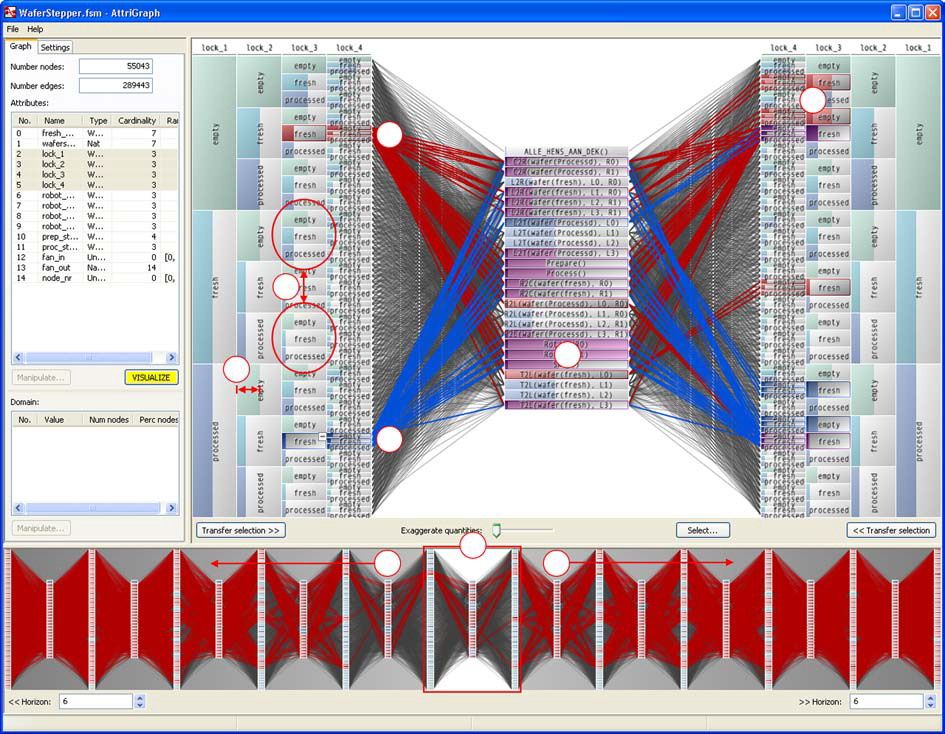
\includegraphics[width=0.95\columnwidth]{figures/MultivariateViz}
  \caption{\label{fig:MultivariateViz} Screen shot taken form Pretorius and Van Wijk's \cite{pretorius2008} multivariate graph visualization application. Permission to be obtained. }
\end{figure}

\paragraph*{Existing Approaches and Techniques}

Pretorius and van Wijk's \cite{pretorius2008} system for visual inspection of multivariate graphs places relationship type (referred to as edge labels) at the core of their system.
They do not use traditional graph layout techniques.
The edges are grouped by label in the center of the display, nodes are duplicated on either side, with the attributes reflected by an icicle plot (see figure \ref{fig:MultivariateViz}).
This approach can handle a large number of edge types, and cases where a node is involved in multiple relationships of different types.

Ghani et al \cite{Ghani2013} developed a techniques called Parallel Node-Link Bands (PNLBs) for exploring graphs with multiple edge types. In their examples edge types are inferred based on their endpoint node types. Nodes are listed in vertical columns with the edges connecting only between neighboring columns.
Is is similar to Pretorious and van Wijk's approach except there are multiple columns of nodes and there is only ever one type of edge between two columns. It is an effective visualization, but is generally limited to smaller data sets and those in which the relationship types are multiple bimodal relationships (as there are no edges drawn between non-adjacent columns).

\subsubsection*{Directed Relationships}

\paragraph*{Description}

While some analyses and datasets involve undirected relationships between genes or gene products, the majority of studies of metabolic networks and other inter-cellular processes rely on directed relationships.
Several researchers that we interviewed stressed the importance of understanding directed relationships between entities.
Depending on the type of relationship in question, edges may be \textit{bi-directional}, which is distinct from an \textit{undirected} edge.
A visual coding that indicates direction must also be able to account for cases in which there are two directional edges between the same two nodes.

\begin{figure}[htb]
  \centering
  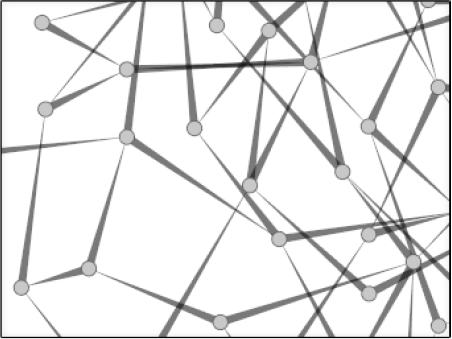
\includegraphics[width=0.8\columnwidth]{figures/tapered_edges}
  \caption{\label{fig:tapered_edges} The tapered directional edges, taken from \cite{Holten2009}. Permission to be obtained. The narrow end of the edge indicates the target.}
\end{figure}

\paragraph*{Existing Approaches and Techniques}

Many visualization applications use the more traditional approach of arrowheads to indicate edge directions, however work by Holten and van Wijk \cite{Holten2009} shows that tapered edges (see fig \ref{fig:tapered_edges}) perform more effectively in conveying edge direction. The graphs used in Holten and van Wijk's were simple directed graphs. Biological pathways are usually modeled as hyper-graphs, with many different types of edge and hyper-edge. Visual encodings such as SBGN and KEGG (see figure \ref{fig:kvik}) contain many different visual representations for edges, so applying the tapered edge visualization style to complex biological pathways is not trivial and would require an empirical evaluation. However, the results of Holten and van Wijk's work suggest that investigating such an approach may be worthwhile.

\subsubsection*{Hierarchical Relationships}

\paragraph*{Description}

Pathway data is inherently hierarchical.
Hierarchical relationships describe relationships of containment, and these relationships can be abstract or based on real biochemical interactions within a cell.
For example, a pathway (itself an abstraction) can be nested within other pathways.
These nested pathways generally encapsulate some commonly-understood hierarchy of biological processes that take place within a cell, such as cellular replication.
Other representations include the more general notion of a ``module'' of connected components, such as gene products.
Hierarchical relationships can also represent physical interactions between biochemical participants.
A common of example of this is in bio-molecular complexes, which are themselves composed of other complexes or biomolecules.

It is important to note that hierarchy and ``structure'' often co-exist with other types of relationships. In most cases, pathway data includes relationships of hierarchy (i.e., when one vertex is contained within another) \textit{in parallel} with other, non-hierarchical relationships, such as the relationship between one gene product that activates or inhibits another. Also, note that while non-hierarchical relationships can take a variety of forms, the only form of hierarchical relationship is one of \textit{containment}, from parent to child, and is undirected.

Hierarchial relationships also include the concept of ``compound'' nodes.
A vertex that contains other entities can be represented as a \textit{compound node}, which is equivalent to a ``parent'' vertex or in some contexts a ``module.'' It is important to note that a one-to-one relationship between an entity and a parent is \textit{not} the same as a one-to-many relationship between an entity and all of that parent's children.
For instance, the \textit{BioPax} format allows for the abstract \emph{NextStep} relationship, which defines, as the name suggests, an arbitrary notion of the ``next step'' of some biological process.
A biochemical reaction could be connected, via a \textit{single} \emph{NextStep} relationship, to an entire pathway, which could potentially contain thousands of nodes.
This relationship is clearly not the same as a biochemical reaction being connected to every entity within a pathway.
This example also demonstrates the distinction between a compound relationship and a hierarchical relationship.
A connection from a node to a compound node does not imply a relationship of ownership or containment.

\begin{figure}[htb]
  \centering
  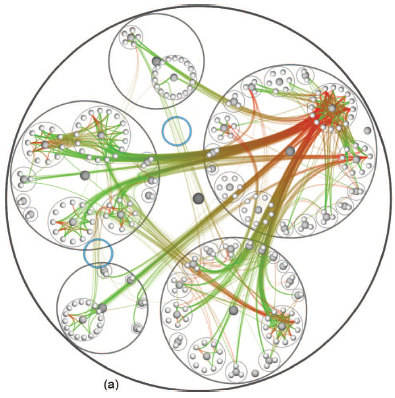
\includegraphics[width=0.5\columnwidth]{figures/Hierarchical_edge_bundles}
  \caption{\label{fig:Hierarchical_edge_bundles} Hierarchical edge bundles, taken from \cite{Holten2006}. Permission to be obtained. The bundles not only reduce clutter but also more clearly define the hierarchy.}
\end{figure}

\paragraph*{Existing Approaches and Techniques}

In terms of visualization there are many techniques for showing hierarchical data.
There are many hierarchical tree based graph layouts that position nodes to emphasis hierarchical nature of data, however these are often not suitable for biological pathway layout as the constrains on position in a layout affect the readability of the lowest level of information.
The RenoDoI application allows for multiple data sources to be included in a single diagram.
This may include data from different pathways and is a containment relationship. Essential the node for each data source forms a set, which may or may not overlap with other sets.
This is visualized using by drawing a bounded contour around the nodes in the set. Different border colors indicate different sets.
This type of encoding of set membership is the \textit{Bubblesets} \cite{Collins2009} approach, which was shown to be the most effective way of displaying group information on a node link diagram by Jianu et al. \cite{Jianu2014}.
\todo[inline]{consider moving previous paragraph to compound Relationships section}

In many cases for pathway visualization the hierarchy is not very deep and edges do not traverse multiple levels of the hierarchy.
However in cases where edges do traverse multiple hierarchical levels they may cause clutter.
Hierarchical Edge Bundling \cite{Holten2006} is a clutter reduction technique, which also emphasizes the hierarchical nature of relationships, see figure\ref{fig:Hierarchical_edge_bundles}. There are many edge bundling techniques in general, however most do not respect hierarchical information during routing.

\subsubsection*{Causality and Cascading Effects}

\paragraph*{Description}

A category of tasks inherent to a variety of work in bioinformatics is the identification of \textit{causal relationships} that exist between bio-molecular entities, and \emph{causal networks} are of particular importance to the analysis of large-scale gene expression data.

When discussing directed paths between entities, one entity is said to be \emph{upstream} or \emph{downstream} of another.
For example, one gene product can increase the activity of other gene products that are \emph{downstream} of it.
Understanding these upstream and downstream relationships is particularly important to domains such as cancer drug research, where a drug may affect a small subset of genes or gene products, which in turn will affect various downstream processes.
In most cases, a directed relationship is meant to represent a biochemical reaction, where one entity is consumed as a reactant and another is produced as a product.
Thus, an upstream entity may be connected to a downstream entity through a chain of several directed links, and a researcher may be interested in understanding the path of reactions (or other relationships) that connects two entities.
However, most cellular processes are inherently complex, and involve many competing sets of directed interactions.
Any given gene is often \textit{mediated} by many different reactants, some which increase activity, and others which decrease activity.
For instance, a causal network helps reveal the likely regulators of a set of genes that are observed to be up-regulated or down-regulated in a particular setting \cite{felciano2013predictive, Kramer2013ipa-causal}.

Thus, determining the set of entities that are ``responsible'' for the increase or decrease in the expression of a particular gene is a challenging task that involves a complex array of directed relationships between many upstream entities.
We characterize this problem as one of identifying \textit{cascading effects}, where many upstream entities have directed relationships with many mediating entities, which in turn affect the output of many downstream entities.

\paragraph*{Existing Approaches and Techniques}

Archambault and Purchase \cite{Archambault2016} have performed a empirical evaluation of different techniques for showing attribute cascades.
They found that visually small multiples was the best approach to convey the dynamic attribute changes that cascade through a network.
The small multiples approach is a form of comparative juxtaposition where multiple views of the network at different time points are displayed in a matrix.
This approach has been used by the cerebral application for showing cascades of data.
Archambault and Purchase's work also shows that layout has an impact on the visualization of attribute cascades.
Experiment participants performed better when a hierarchical layout was used, however it should be noted that the hierarchical layout was consistent with the direction of the layout.

\todo[inline, author=FMG]{I think it would be a good idea to differentiate this taxonomy from Ahn's taxonomy in this section. He does look at causal tasks and repetition, which are related to feedback loops , but not the same....}

\subsubsection*{Feedback Loops}

\paragraph*{Description}

In tandem with the problem of identifying cascading effects is the problem of reasoning with feedback.
Feedback loops are common within metabolic activation networks, and they play a key role in processes related to uncontrolled cellular growth in cancerous cells.

\paragraph*{Existing Approaches and Techniques}

\hl{to do}

\subsection*{Comparisons and Contextualization}

\paragraph*{Description}

Related to the issue of multivariate attributes is the need to compare related pathways or sets of entities, or to compare a given pathway across a number of states.
For instance, microarray measurements are often used to measure gene expression levels for a control group and an experimental group over several time steps.
The goal of this research is to discover significant empirical differences between groups and across time, and the visual comparison of these groups is useful.

The topic of contextualization includes a very important component of modern biology, which is the incorporation of multiple external datasets.
Biological pathway data is inherently large, complex, and subject to ongoing contributions from contemporary research.
Thus, for biological pathway visualization in particular, integration of attribute data from external data sources is essential.

\hl{both an issue of performance and in integrating with external community resources}

\paragraph*{Existing Approaches and Techniques}

Most applications provide access to the attributes through simple interactions (e.g.~mouseover and click).
In many cases the attribute information is simply read from an input file, however more recent tools such as \textit{SBGNViz} \cite{SBGNViz2015} and \textit{ChiBE}\cite{Babur2010chibe} query online database to provide a range of important attribute information.

In their 2011 survey Gleicher et al. \cite{Gleicher2011} describe three primary types classifications of comparative visualization.
These are juxtaposition, superposition, and explicit encoding of differences, and these classifications can also be combined.
Juxtaposition is when the visualizations being compared are displayed side by side.
This is functionality is available by default in Cytoscape (and hence all of the associated plug-ins).
Cerebral uses a juxtaposition approach to display changes in attributes associated with the graph.

Superposition is when is when data sets are displayed as part of the same visualization.
The RenoDoI plugin also offers superposition , allowing multiple networks to be visualized in the one image. Bounding isocountours are used to distinguish graphs differences, and to clearly indicate where the graphs overlap.
Graph layout is and important aspect of both juxtaposition and superposition based comparative visualizations.
For juxtaposition, the two graphs being compared should have as similar layout in possible , to aid comparison.
For supposition, the matter is not so simple as the addition of a new graph may destroy the existing layout.
The RenoDoI application\cite{Vehlow2015} initially lays out the largest data set, then adds the addition data sets, adjusting previous layout , without resetting it.
Nodes which are included in both data sets only appear once.

Explicit encoding of difference means that differences between the two datasets are explicitly highlighted, and this approach is often in addition to the previous two.
Once specific case where implicit encoding is not mixed is when when a graph is dynamic and the changes are between time slices.
This can be seen in Rugfiange and McGuffins's DiffAni application \cite{Rufiange2013}.

\subsection*{Data Modification and Curation}

\paragraph*{Description}

While most of the tasks in this taxonomy are directly related to visual analysis, the size and complexity of biological datasets makes data curation an essential part of modern research platforms.
Several of the researchers we interviewed mentioned certain tasks related to the curation, maintenance, and understanding of pathway data.
For instance, one researcher mentioned the importance of being able to \emph{debug} potentially flawed data.
Two others expressed a need to create ``personalized'' pathways that only include a user-determined subset of entities and relationships.

Ideally, visualization tools will seamlessly integrate these curation and maintenance needs.

\paragraph*{Existing Approaches and Techniques}

\hl{to do}

\subsection*{Discussion}

\subsection*{Directions for Future Research}

\subsubsection*{Visualizing Uncertainty}

Especially considering our feedback from domain experts, tools generally do not attempt to visualize the ``uncertainty'' behind a connection in a pathway, as expressed by the first domain expert. This is a challenging task, as even the definition of ``uncertainty'' may be difficult to operationalize. However, data formats such as \emph{BioPAX} do have robust support for citations, allowing published references to be connected to entities and relationships within a pathway. A tool that could effectively encode ``uncertainty data'' into a visualization may be very valuable to systems researchers who work with the results of hundreds or thousands of separate publications.

\section*{Conclusions}
